\section{Methodology}

\subsection{Machine Learning Approach}

In this study, many different approaches were attempted and compared to extract meaningful features from the images and compute the appropriate morphological properties of the dune fields. The approach presented in this paper can be summarized as a five stage process:

\begin{enumerate}
	\item Image Preprocessing
	\item Dominant Orientation Determination
	\item Crest-line Candidate Detection
	\item Validation
	\item Metrics Calculations
\end{enumerate}

\subsubsection{Image Preprocessing}

The pre-processing stage is an important step to normalize and de-noise the input data. Image processing is typically a low level process which attempts to improve image quality, normalize illumination, or remove unnecessary information from the image. This type of processing will in turn improve higher level feature extraction.

The first step is to insure that the images have roughly the same scale. To enforce scale normalization, the datasets scales were manually selected for appropriate crest-line detection application, and the image resolutions were resized to roughly 1000 pixel in width. The appropriate resolution is chosen based on a few factors:

\begin{itemize}
	\item Source resolution: The selected resolution is limited by the original image's resolution. No extra information can be gained from increasing the source image's resolution.
	\item Processing time: Higher resolution images require much more processing time overall which could be a limitation in a certain application.
	\item Scale selection: If the application's domain is found in a higher scale space, a higher resolution may not necessarily be required.
\end{itemize}

In this application, the goal is to detect the major crest-line, which is a higher scale domain, which means a higher resolution image is not a necessity. Note that some of the parameter selection in these processes are dependent on the resolution and scale of the images. In future work, dominant scale of the crest-lines could be determined automatically to improve the robustness of the algorithms.

The next step in the process is to convert the images to gray scale. The images in the terrestrial, and Ganges datasets (described in section \ref{subsec:terrestrial_dataset} and \ref{subsec:mars_dataset}) are color images by default. Although color processing of these images has not extensively been tested as part of this study, it is arguable whether using color information would improve the detection results. By converting the images to gray scale, an added benefit of normalizing the images across many region is implicitly enforced. Finally, the conversion process turns the three channel image into a single channel image which improves overall processing performance.

The final preprocessing step is to improve the image quality with low-pass filters. Many of the algorithms in this method rely on gradient information. Therefore, to extract the meaningful gradients, removing the highest frequencies (which in typically are responsible for noise), while preserving the lower scale or more desirable gradients. Two main popular filters are utilized. The median filter, introduced in \cite{huang_median_filtering_algorithm}, is applied first to remove grain and salt and pepper noise while preserving important edges. In some cases, median filtering also helps remove some smaller scale objects such as bushes, trees, rocks, and other features which are indistinguishable from satellite images. Following is the standard Gaussian filter which removes the remaining high frequency noisy signals from the image.

An important aspect to note is the size of the filter masks, which is heavily dependent on the resolution of the input image. We found that in most cases, for images around 1000 pixels in width, a \emph{sigma} value of approximately 1.5 and mask size of 7 by 7 was sufficient for this application. Once the image has been preprocessed, the gradients can be computed and saved for future use. Gradients can be computed by taking the first derivative of the image, using the popular Sobel operator.

An optional additional step is to apply histogram equalization to the image \cite{digital_image_processing_book}. Poorly illuminated or low contrast images greatly benefit from histogram equalization, because it stretches the contrast of the image in a consistent way. Using this process has shown to improve the overall results in many cases. 

\subsubsection{Dominant Orientation Determination}

Computing the dominant orientation of the dune field is an important step in the process. The dominant orientation is the gradient direction of the crest-lines to be detected. This process can help determine the average orientation of the dune field as well. 

An important point to make is that this process could be optional if the dominant orientation is known a priori. Working with a dataset where the values are known improves the overall results of detection and enables skipping of this step. In cases where this information is unknown, or unavailable, automated dominant orientation determination is a potential solution.

Typically, there exists a gradient peak at the crest-line peak of the dunes (although this may not always be the case for less pronounced dunes). The direction of the gradient should agree with the overall dominant orientation of the dune field. Computing the dominant orientation of the field can be challenging in many cases because dunes typically have two major orientations, which are opposite directions. This phenomenon is clearly illustrated in Figure \ref{fig:computing_dominant_orientation}. The true crest-line peak, where the sunny side meets the shaded side is one gradient (fig. \ref{fig:true_dominant_orientation_image}). At the foot of the dune, where the shaded returns to light, a second gradient will be present, whom has an opposite direction (fig. \ref{fig:false_dominant_orientation_image}).

\begin{figure}
	\centering
	\begin{subfigure}{0.48\textwidth}
		\centering
		\includegraphics[width=\linewidth]{figures/dominant_orientation_false}
		\caption{}
		\label{fig:false_dominant_orientation_image}
	\end{subfigure}
	\begin{subfigure}{0.48\textwidth}
		\centering
		\includegraphics[width=\linewidth]{figures/dominant_orientation_true}
		\caption{}
		\label{fig:true_dominant_orientation_image}
	\end{subfigure}
	\begin{subfigure}{\textwidth}
		\centering
		\includegraphics[width=0.8\linewidth]{figures/dominant_orientation_histogram}
		\caption{}
		\label{fig:dominant_orientation_histogram}
	\end{subfigure}
	
	\caption{Results of unnormalized (red) and normalized (green) histograms of gradients ($N=18$). The histogram contains two major peaks, but the crest-line is the weaker of the two peaks. (a) Edges which belong to the dominant orientation which are invalid crest-lines. (b) With normalization, the true crest-lines now have the higher overall magnitude. (c) The 18 bin histogram of gradients with and without normalization.}
	\label{fig:computing_dominant_orientation}
\end{figure}

To remedy this issue, using histograms of gradient directions can be used to determine the true orientation. Histograms have been used for many processes and applications including \cite{lowe_sift_paper, dalal_histogram_oriented_gradients_human_detection, hu_gradient_field_descriptor}. Quantizing the space allows us to split edges according to their orientation, where each bin in the histogram represents an edge orientation. Each bin then covers an angle of $\frac{2\pi}{N}$radians, where \emph{N} is the number of bins. Each bin of the histogram is weighed by the magnitude of edges. Once the histogram is constructed, peaks in the magnitude
will help determine the dominant orientation ($\varPhi$) of the dune
crest-lines. The approach poses two main problems:

\begin{enumerate}
	\item Determining \emph{N}: In practice, a larger value for \emph{N} has shown to provide finer grain resolution which improves dominant orientation determination. In Figure \ref{fig:computing_dominant_orientation} a value of $N=18$ is used.
	\item Multiple Peaks: Often, images may have multiple peaks
	in the histogram, but only one of the peaks should represents the
	true dominant orientation of crest-lines.
	\item Global Solution: The computed dominant orientation is global to the image, which may not be optimal in cases of complex dune structures. A better solution would be to compute the dominant orientation in a local area of the image, to account for local shifts in orientation.
\end{enumerate}

One assumption made is that the bin with the largest value represents the orientation of the crest-line edges. Although this assumption holds for many cases, it is not always the case. The Skeleton Coast test image provides a good example of this case in Figure \ref{fig:computing_dominant_orientation}. In this particular case, the are two major peaks in the histogram, where the stronger is not the part of the crest-line edge group, and the weaker one is. Choosing the higher peak will cause invalid crest-lines to be chosen. In order to determine which peak best represents the crest-line edge group, some normalization can be applied. The normalization process begins by computing the mean vector of the gradients from the edge image as follows:

\[
\hat{\mu}\left\langle \bar{x},\bar{y}\right\rangle =\left\langle \frac{\sum_{i=0}^{P}\delta_{x_{i}}}{P},\frac{\sum_{i=0}^{P}\delta_{y_{i}}}{P}\right\rangle 
\]

where \emph{P} is the total number of detected edges from the Canny edge detector, $\delta_{x_{i}}$ and $\delta_{y_{i}}$ are the \emph{x} and \emph{y} gradient component of the \emph{i}\textsuperscript{th} point. The
mean orientation is computed from the mean vector as:

\[
\bar{\theta_{\mu}}=\arctan\left(\frac{\mu_{\bar{y}}}{\mu_{\bar{x}}}\right)
\]

The gradients are then normalized by simply subtracting the mean vector from each gradient:

\[
\dot{\delta}\left(x_{i},y_{i}\right)=\left(\delta_{x_{i}}-\mu_{\bar{x}},\delta_{y_{i}}-\mu_{\bar{y}}\right)
\]

The normalized orientation $\dot{\theta_{i}}$ can be computed:

\[
\dot{\theta_{i}}=\arctan\left(\frac{\dot{\delta_{y_{i}}}}{\dot{\delta_{x_{i}}}}\right)
\]

To determine which bin the \emph{i}\textsuperscript{th}	edge point belongs to, we simply calculate $\left\lceil \frac{\dot{\theta_{i}}\centerdot N}{2\pi}-0.5\right\rceil $,	and increment that bin by the magnitude of the normalized gradient	by $\sqrt{\dot{\delta}_{x_{i}}^{2}+\dot{\delta}_{y_{i}}^{2}}$. In essence, this normalization process removes the uneven skew of the gradients in the overall image. Removing this skew allows true crest-line edges to be fairly compared with other stronger edges. As shown in Figure \ref{fig:computing_dominant_orientation}, the normalization process softens the stronger dominant edge and enhances the true crest-line edges. This process enables true crest-lines to be accurately determined in images where the valleys of dunes are sharp and contain strong edges.

Once the histogram is computed and normalized, the dominant orientation vector $\hat{\theta_{dom}}$ is determined by averaging the gradients belonging to the histogram bin with the highest value. With the dominant orientation knowledge acquired, candidate crest-line dunes can be detected.

\subsubsection{Crest-line Candidate Detection}  

The goal of the initial candidate detection step is to find as many of the true crest-lines as possible. For optimal results, candidate detections should span as much of the crest-line as possible and ideally be a single contiguous segment. These constraints help improve the overall accuracy and compute the geomorphological properties of the dune fields.

The candidate detection process can be summarized in four steps:

\begin{enumerate}
	\item Compute the gradient orientation image relative to the dominant orientation.
	\item Threshold the gradient orientation image to preserve all pixels which agree with the dominant orientation.
	\item Find the contours of the thresholded regions of the gradient orientation image.
	\item Shift the contours to the nearest gradient magnitude peak.
\end{enumerate}

The relative gradient orientation image maps the gradient directions relative to the computed dominant orientation. This can be achieved by taking the dot product of the normalized gradient vectors, with the normalized dominant orientation vector at each pixel location on the image, as shown below.
\[
R_{\theta_{ij}} = \hat{\delta_{ij}}\cdot \hat{\theta_{dom}}
\]

In essence, the resulting image $R_{\theta}$ displays maps the gradient direction vectors to a single value with a range of values from $-1$ to $+1$. A brighter pixel then \emph{agrees} with the dominant orientation while dark pixels \emph{disagrees} with it. The resulting transformation is shown in Figure \ref{fig:gradient_direction_image_transformation}.

\begin{figure}
	\centering
	\begin{subfigure}{0.48\textwidth}
		\centering
		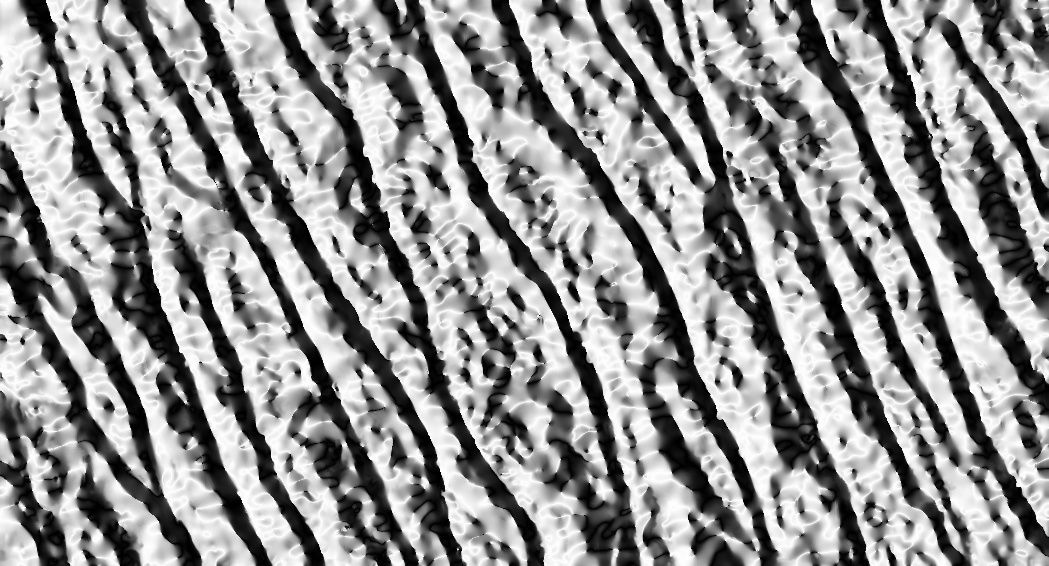
\includegraphics[width=\linewidth]{figures/gradient_direction_image}
		\caption{}
		\label{fig:gradient_direction_image}
	\end{subfigure}
	\begin{subfigure}{0.48\textwidth}
		\centering
		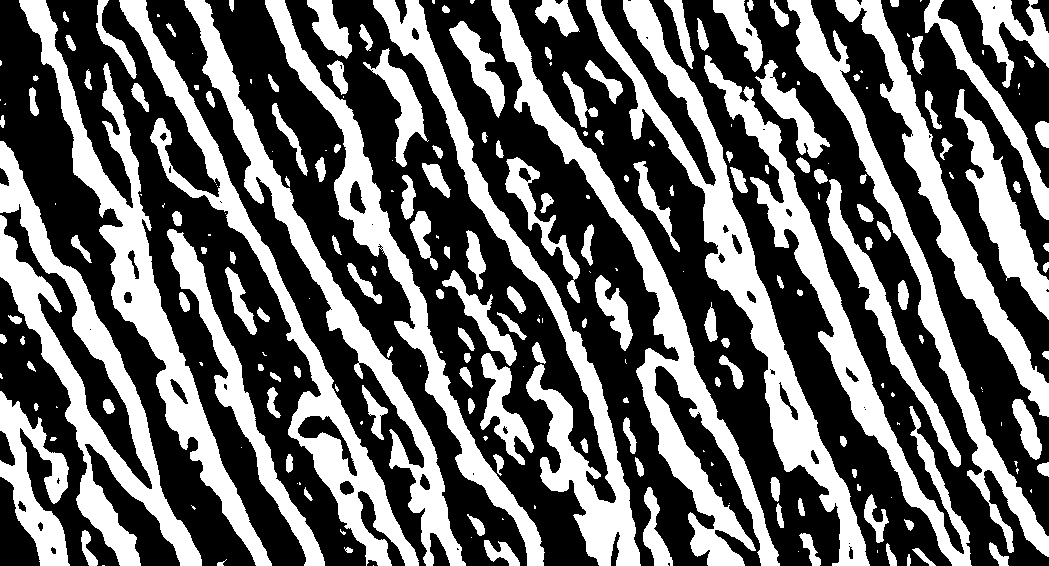
\includegraphics[width=\linewidth]{figures/gradient_direction_thresholded_image}
		\caption{}
		\label{fig:gradient_direction_thresholded_image}
	\end{subfigure}
	\caption{}
	\label{fig:gradient_direction_image_transformation}
\end{figure}

The benefit of this transformation is that due to the nature of the domain problem, this produces bright regions around dune crest-lines. Another benefit is that it much less sensitive to weaker  